% 原书印刷202--207页，PDF物理226--231页，止于5.5标题之前.
\subsection[Wasserstein空间中的常速测地线]{$\mathbb W_p$中的常速测地线}\label{sec:5.4}\index{D043@位移插值（displacement interpolation）|hyperpage}

本节将看到$\mathbb W_p$中的常速测地线如何与最优运输映射相联系. 在此之前，先回顾度量空间中测地线的主要事实.

\begin{sourcebox}{相关知识：一般度量空间中的常速测地线}\label{box:5.2}\index{G065@测地线（geodesics）!068@度量空间中（in metric spaces）|hyperpage}
首先定义一般度量空间$(X,d)$中曲线$\omega$的长度.
\begin{definition*}
对曲线$\omega:[0,1]\to X$，定义
\[
\operatorname{Length}(\omega):=\sup\left\{\sum_{k=0}^{n-1}d(\omega(t_k),\omega(t_{k+1})):
n\ge1,\ 0=t_0<t_1<\cdots<t_n=1\right\}.
\]
\end{definition*}
注意，同一定义也可用于定义在$[0,1]$、取值于$X$而不一定连续的函数. 满足$\operatorname{Length}(\omega)<+\infty$的函数$\omega$，恰好是一维BV函数意义下具有有界变差的函数（见\autoref{sec:4.2.4}的\autoref{box:4.4}）. 容易看出，所有曲线$\omega\in\mathrm{AC}(X)$均满足$\operatorname{Length}(\omega)\le\int_0^1g(t)\,dt<+\infty$.
\begin{proposition*}
对任意曲线$\omega\in\mathrm{AC}(X)$，有
\[
\operatorname{Length}(\omega)=\int_0^1|\omega'|(t)\,dt.
\]
\end{proposition*}
再列出一些定义.
\begin{definition*}
若曲线$\omega:[0,1]\to X$在所有满足$\omega(0)=x_0$与$\omega(1)=x_1$的曲线中使长度最小，则称其为$x_0$与$x_1\in X$之间的\emph{测地线}（geodesic）.

若空间$(X,d)$满足
\[
d(x,y)=\inf\{\operatorname{Length}(\omega):\omega\in\mathrm{AC}(X),\ \omega(0)=x,\ \omega(1)=y\},
\]
则称它为\emph{长度空间}（length space）.

若空间$(X,d)$满足
\[
d(x,y)=\min\{\operatorname{Length}(\omega):\omega\in\mathrm{AC}(X),\ \omega(0)=x,\ \omega(1)=y\},
\]
则称它为\emph{测地空间}（geodesic space），即它是长度空间，而且任意两点之间存在测地线.
\end{definition*}
这里不详细讨论测地线存在的条件，但$\operatorname{Length}(\omega)$定义为一个上确界这一点，对建立半连续性结果至关重要.

\begin{definition*}
在长度空间中，若曲线$\omega:[0,1]\to X$满足
\[
d(\omega(t),\omega(s))=|t-s|d(\omega(0),\omega(1))\qquad\text{对所有 }t,s\in[0,1],
\]
则称它为$\omega(0)$与$\omega(1)\in X$之间的\emph{常速测地线}（constant-speed geodesic）.
\end{definition*}
容易验证，具有此性质的曲线自动是测地线. 以下刻画很有用.
\begin{proposition*}
固定指数$p>1$，考虑连接$x_0$与$x_1$的曲线. 以下三件事等价：
\begin{enumerate}
\item $\omega$是常速测地线；
\item $\omega\in\mathrm{AC}(X)$且几乎处处有$|\omega'|(t)=d(\omega(0),\omega(1))$；
\item $\omega$解出$\min\{\int_0^1|\omega'|(t)^p\,dt:\omega(0)=x_0,\ \omega(1)=x_1\}$.
\end{enumerate}
\end{proposition*}
\end{sourcebox}

先证明，若$\Omega$凸，则空间$\mathbb W_p(\Omega)$是长度空间.

\begin{theorem}\label{obj:5.27}\index{G065@测地线（geodesics）!066@$\mathbb W_p$中（in $\mathbb W_p$）|hyperpage}
假设$\Omega$凸，取$\mu,\nu\in\mathscr P_p(\Omega)$，以及成本$c(x,y)=|x-y|^p$（$p\ge1$）的最优运输方案$\gamma\in\Pi(\mu,\nu)$. 通过$\pi_t(x,y)=(1-t)x+ty$定义$\pi_t:\Omega\times\Omega\to\Omega$. 则曲线$\mu_t:=(\pi_t)_\#\gamma$是$\mathbb W_p$中连接$\mu_0=\mu$与$\mu_1=\nu$的常速测地线.

特别地，若$\mu$绝对连续，或更一般地，若$\gamma=\gamma_{\mathrm T}$，则这一曲线由$((1-t)\mathrm{id}+t\mathrm T)_\#\mu$给出.

因而空间$\mathbb W_p(\Omega)$是测地空间.
\end{theorem}
\begin{proof}
只需证明$W_p(\mu_t,\mu_s)\le W_p(\mu,\nu)|t-s|$. 事实上，假设对每个$s>t$均已证明，则有
\[
\begin{aligned}
W_p(\mu,\nu)&\le W_p(\mu,\mu_t)+W_p(\mu_t,\mu_s)+W_p(\mu_s,\nu)\\
&\le W_p(\mu,\nu)(t+(s-t)+(1-s))=W_p(\mu,\nu),
\end{aligned}
\]
所以所有不等式均为等式. 为证明断言，取$\gamma_t^s:=(\pi_t,\pi_s)_\#\gamma\in\Pi(\mu_t,\mu_s)$，计算
\[
\begin{aligned}
W_p(\mu_t,\mu_s)&\le\left(\int|x-y|^p\,d\gamma_t^s\right)^{1/p}
=\left(\int|\pi_t(x,y)-\pi_s(x,y)|^p\,d\gamma\right)^{1/p}\\
&=|t-s|\left(\int|x-y|^p\,d\gamma\right)^{1/p}=|t-s|W_p(\mu,\nu),
\end{aligned}
\]
这里使用了$|(1-t)x+ty-(1-s)x-sy|=|(t-s)(x-y)|$.
\end{proof}

\phantomsection\label{idx:root5-p203-bb}\index{B015@Benamou--Brenier方法（Benamou-Brenier）|hyperpage}分析$\mathbb W_p$中的常速测地线之前，强调测地空间性质与\autoref{obj:5.14}的一个重要推论. 这一结果通常称为\emph{Benamou--Brenier公式}，可视为Kantorovich问题的动态版本，其背后的想法将在\autoref{sec:6.1}提供数值刻画时起关键作用.

\begin{theorem}\label{obj:5.28}
在凸紧区域$\Omega$上，给定$\mu,\nu\in\mathscr P(\Omega)$，有
\[
W_p^p(\mu,\nu)=\min\{\mathscr B_p(\varrho,E):\partial_t\varrho+\nabla\cdot E=0,\ \varrho_0=\mu,\ \varrho_1=\nu\},
\]
其中$\varrho$与$E$都应视为时空$\Omega\times[0,1]$上的测度.
\end{theorem}
\begin{proof}
由于$\mathbb W_p$是长度空间，
\[
W_p^p(\mu,\nu)=\left(\min\left\{\int_0^1|\varrho'|(t)\,dt:\varrho_0=\mu,\ \varrho_1=\nu\right\}\right)^p.
\]
可将极小化限制于常速测地线；由\autoref{box:5.2}给出的刻画，还得到
\[
W_p^p(\mu,\nu)=\min\left\{\int_0^1|\varrho'|(t)^p\,dt:\varrho_0=\mu,\ \varrho_1=\nu\right\}.
\]
再使用\autoref{obj:5.14}，将$|\varrho'|(t)$替换为$\|\mathbf v_t\|_{L^p(\varrho_t)}$，得到
\[
W_p^p(\mu,\nu)=\min\left\{\int_0^1\|\mathbf v_t\|_{L^p(\varrho_t)}^p\,dt:
\partial_t\varrho_t+\nabla\cdot(\varrho_t\mathbf v_t)=0,\ \varrho_0=\mu,\ \varrho_1=\nu\right\}.
\]
令$E_t=\varrho_t\mathbf v_t$，陈述只是上述公式的改写.
\end{proof}

回到$\mathbb W_p$中测地线的结构，并再次记住\autoref{obj:5.14}的重要结果，可以问，与这些测地线相应的速度场是什么. 事实上，常速测地曲线$\mu_t$为Lipschitz曲线，因而必有速度场$\mathbf v_t$（至少当$p>1$时），满足连续性方程$\partial_t\mu_t+\nabla\cdot(\mu_t\mathbf v_t)=0$.

粗略说来，就是对$t\in]0,1[$，取$y\in\operatorname{spt}(\mu_t)\subset\Omega$，尝试寻找时刻$t$经过$y$的粒子的速度. 这应当就是$\mathbf v_t(y)$的值. 若在时刻$t$经过$y$的“粒子”唯一，就更容易回答这一问题. 通过下述引理获得唯一性.

\begin{lemma}\label{obj:5.29}
设$\Omega$紧，$\gamma$是两个概率测度$\mu,\nu\in\mathscr P(\Omega)$之间成本$c(x,y)=h(y-x)$的最优运输方案，其中$h$严格凸；取$t\in]0,1[$. 令$\mu_t=(\pi_t)_\#\gamma$，其中$\pi_t(x,y)=(1-t)x+ty$，并取$y\in\operatorname{spt}(\mu_t)$. 则存在唯一一对$(x,z)\in\operatorname{spt}(\gamma)$，使$y=(1-t)x+tz$. 将这些$x,z$的值分别记作$X_t(y)$与$Z_t(y)$. 映射$X_t$与$Z_t$还连续.

特别地，若$\gamma=\gamma_{\mathrm T}$来自运输映射，则映射$\mathrm T_t:=(1-t)\mathrm{id}+t\mathrm T$可逆，且$\mathrm T_t^{-1}=X_t$.
\end{lemma}
\begin{proof}
断言与\autoref{obj:4.23}中的断言本质相同，$(x,z)\in\operatorname{spt}(\gamma)$的唯一性来自$\operatorname{spt}(\gamma)$的$c$-循环单调性. $X_t$与$Z_t$的连续性通过紧性得到. 取$y_n\to y$，假设取子列后$(X_t(y_n),Z_t(y_n))\to(X,Z)$. 因$\operatorname{spt}(\gamma)$闭，$(X,Z)\in\operatorname{spt}(\gamma)$. 再由唯一性，$(X,Z)=(X_t(y),Z_t(y))$. 由于任意收敛子列的极限都必须与$y$处的值一致，且所在空间紧，就得到连续性.
\end{proof}

现在可以确定测地线$\mu_t$的速度场：已知每个初始位于$x$的粒子沿直线以常速度$\mathrm T(x)-x$运动，这蕴含$\mathbf v_t(y)=(\mathrm T-\mathrm{id})(\mathrm T_t^{-1}(y))$. 更一般地，若$\gamma$不由映射诱导，则$\mathbf v_t(y)=Z_t(y)-X_t(y)$.

\begin{proposition}\label{obj:5.30}
设$\mu_t=(\pi_t)_\#\gamma$为上面介绍的连接$\mu$与$\nu$的测地线. 则对每个$t\in]0,1[$，速度场$\mathbf v_t:=Z_t-X_t$在$\operatorname{spt}(\mu_t)$上有良好定义，且满足
\[
\partial_t\mu_t+\nabla\cdot(\mu_t\mathbf v_t)=0,
\qquad\|\mathbf v_t\|_{L^p(\mu_t)}=|\mu'|(t)=W_p(\mu,\nu).
\]
\end{proposition}
\begin{proof}
已知$X_t$与$Z_t$有良好定义，因而只需验证连续性方程与$L^p$估计. 为证明连续性方程，取$\phi\in C^1$，计算
\[
\begin{aligned}
\frac d{dt}\int\phi\,d\mu_t
&=\frac d{dt}\int\phi((1-t)x+tz)\,d\gamma(x,z)\\
&=\int\nabla\phi((1-t)x+tz)\cdot(z-x)\,d\gamma(x,z)\\
&=\int\nabla\phi(\pi_t(x,z)\cdot(Z_t(\pi_t(x,z))-X_t(\pi_t(x,z))))\,d\gamma(x,z)\\
&=\int\nabla\phi(y)\cdot(Z_t(y)-X_t(y))\,d\mu_t(y).
\end{aligned}
\]
为计算$L^p$范数，有
\[
\int|\mathbf v_t|^p\,d\mu_t
=\int|Z_t(y)-X_t(y)|^p\,d\mu_t(y)
=\int|z-x|^p\,d\gamma(x,z)=W_p^p(\mu,\nu).
\]
两项计算都利用了每个$(x,z)\in\operatorname{spt}(\gamma)$满足$Z_t(\pi_t(x,z))-X_t(\pi_t(x,z))=z-x$这一事实.
\end{proof}

\phantomsection\label{idx:root5-p205-kinetic}\index{K085@动能（kinetic energy）|hyperpage}\index{M098@曲线上的测度（measures on curves）|hyperpage}现在要证明，至少当$p>1$时，距离$W_p$的全部测地线均有此形式，即都由某个最优$\gamma$按$\mu_t=(\pi_t)_\#\gamma$给出. 若$\gamma$不唯一，测地线也仍不唯一. 这里的证明不同于\cite{b15}，并基于下述表示定理（具有\cite{b212}的精神）. 使用定义在$[0,1]$、取值于$\Omega$的绝对连续曲线集合$\mathrm{AC}(\Omega)$，用$K_p:\mathrm{AC}(\Omega)\to\mathbb R\cup\{+\infty\}$表示$p$-动能，定义为$K_p(\omega):=\int_0^1|\omega'(t)|^p\,dt$（仅当$\omega$属于Sobolev空间$W^{1,p}([0,1])\subset\mathrm{AC}(\Omega)$时才有限）. 与通常一样，简记$\mathscr C=\mathrm{AC}(\Omega)$.

\begin{proposition}\label{obj:5.31}
对$\mathbb W_p(\Omega)$中的每条Lipschitz曲线$(\mu_t)_t$，存在测度$Q\in\mathscr P(\mathscr C)$，使$\mu_t=(e_t)_\#Q$且$\int_{\mathscr C}K_p(\omega)\,dQ(\omega)\le\int_0^1|\mu'|(t)^p\,dt$.
\end{proposition}
\begin{proof}
先注意，由\autoref{obj:5.14}，对几乎每个$t$，存在向量场$\mathbf v_t\in L^p(\mu_t)$，使$\partial_t\mu_t+\nabla\cdot(\mathbf v_t\mu_t)=0$，且$\|\mathbf v_t\|_{L^p(\mu_t)}\le|\mu'|(t)$. 使用与\autoref{obj:5.14}中相同的逼近论证（及相同卷积核），得到正则化测度曲线$\mu_t^\varepsilon$与正则化向量场$\mathbf v_t^\varepsilon$，其中$\|\mathbf v_t^\varepsilon\|_{L^p(\mu_t^\varepsilon)}\le\|\mathbf v_t\|_{L^p(\mu_t)}$. 这一向量场具有流$Y:\Omega\to\mathrm{AC}(\Omega)$，其中$Y(x)$为曲线$y_x(\cdot)$，且已知$\mu_t^\varepsilon=(Y_t)_\#\mu_0^\varepsilon$，$Y_t(x)=Y(x)(t)=y_x(t)$. 再定义测度$Q^\varepsilon:=Y_\#\mu_0^\varepsilon$. 有$\mu_t^\varepsilon=(e_t)_\#Q^\varepsilon$.

计算$\int_{\mathscr C}K_p\,dQ^\varepsilon$：
\[
\begin{aligned}
\int_{\mathscr C}K_p(\omega)\,dQ^\varepsilon(\omega)
&=\int_\Omega\int_0^1|\mathbf v_t^\varepsilon(y_x(t))|^p\,dt\,d\mu_0^\varepsilon(x)
=\int_0^1\int_\Omega|\mathbf v_t^\varepsilon|^p\,d\mu_t^\varepsilon\\
&\le\int_0^1\int_\Omega|\mathbf v_t|^p\,d\mu_t
=\int_0^1|\mu'|(t)^p\,dt.
\end{aligned}
\]
现在（如\autoref{sec:4}中多次所见），这意味着测度$Q^\varepsilon$一致紧，因为$\int_{\mathscr C}K_p\,dQ^\varepsilon$有界，而且对每个$L$，集合
\[
\{\omega\in\mathrm{AC}(\Omega):K_p(\omega)\le L\}
\]
在$C^0([0,1])$中关于一致收敛紧. 此外，$K_p$对同一种收敛下半连续. 因而可找到子列，使$Q^\varepsilon\rightharpoonup Q$，且$\int_{\mathscr C}K_p\,dQ\le\liminf_\varepsilon\int_{\mathscr C}K_p\,dQ^\varepsilon$. 由$\mu_t^\varepsilon=(e_t)_\#Q^\varepsilon$，得到$\mu_t=(e_t)_\#Q$，结论成立.
\end{proof}

\begin{proposition}\label{obj:5.32}
设$(\mu_t)_t$是$\mathbb W_p(\Omega)$中$\mu$与$\nu$之间的常速测地线，且$p>1$. 则对于运输成本$c(x,y)=|x-y|^p$，存在最优$\gamma\in\Pi(\mu,\nu)$，使每个$t\in[0,1]$均有$\mu_t=(\pi_t)_\#\gamma$.
\end{proposition}
\begin{proof}
由于曲线为常速测地线，对几乎每个$t$有$|\mu'|(t)=W_p(\mu,\nu)$（度量导数按$W_p$计算）. 应用前面的\autoref{obj:5.31}，得到测度$Q\in\mathscr P(\mathscr C)$，满足$\mu_t=(e_t)_\#Q$与$\int_{\mathscr C}K_p(\omega)\,dQ(\omega)\le\int_0^1|\mu'|(t)^p\,dt$.

由Jensen不等式，$|\omega(0)-\omega(1)|^p\le K_p(\omega)$，且等号当且仅当$\omega$是以常速参数化的线段. 因而
\[
\begin{aligned}
W_p^p(\mu,\nu)&\le\int_{\mathscr C}|\omega(0)-\omega(1)|^p\,dQ(\omega)\\
&\le\int_{\mathscr C}K_p(\omega)\,dQ(\omega)
\le\int_0^1|\mu'|(t)^p\,dt\le W_p^p(\mu,\nu).
\end{aligned}
\]
第一个不等式来自$\gamma:=(e_0,e_1)_\#Q\in\Pi(\mu_0,\mu_1)$；第二个来自上述关于$K_p$的不等式；最后一个来自$Q$的性质. 因而所有不等式都是等式. 所以$Q$集中于常速线段曲线，且$\gamma$为最优运输方案. 这证明了$\mu_t=(\pi_t)_\#\gamma$.
\end{proof}

注意，上述证明与\autoref{obj:4.13}的证明相似，只是这里为动态框架，而\autoref{sec:4}中是静态框架.

不难看出，\autoref{obj:5.31}与\autoref{obj:5.32}在$p=1$时都不成立. 反例如常，仍由$\mu_t=(1-t)\delta_{x_0}+t\delta_{x_1}$给出.

最后强调Wasserstein测地线在应用中的作用：它们通过将粒子从一个分布缓慢移动到另一个分布，在两个质量分布（或两个直方图）之间构造有趣的插值. 例如，\autoref{fig:5.2}显示\autoref{fig:2.4}中色度直方图之间的插值. 这些中间直方图还可以用于生成中间图像.

\begin{figure}[htbp]
\centering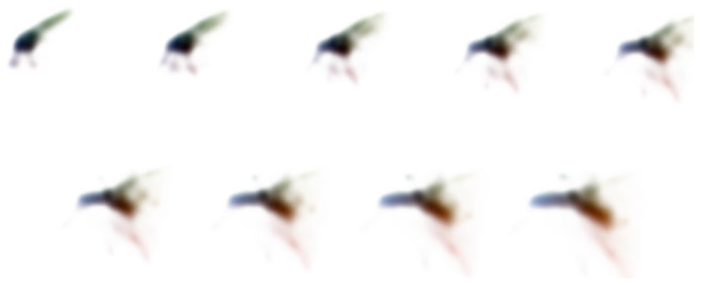
\includegraphics[width=\linewidth]{assets/ch05-fig-5-2.pdf}
\caption{通过$\mathbb W_2$测地曲线，在\autoref{fig:2.4}两张图像的二维色度信号空间直方图之间得到的九个插值时刻（上排从左到右，再下排从左到右）. 图片由G.~Peyré惠予提供.}\label{fig:5.2}
\end{figure}
